% !TEX root = ../latexnote.tex
\chapter{正文工具}\label{chap:text}
\section{章节}\label{sec:section}

一篇结构化的、条理清晰文档一定是层次分明的,通过不同的命令分割为章、节、小节。三个标准文档类 article、report 和 book\footnote{千万注意是标准文档类,其它文档类,如果不是从标准文档类衍生而来,很可能没有定义或只定义了一部分命令}提供了划分章节的命令:
\begin{lstlisting}
\chapter{章名}
\section{节名}
\subsection{小节名}
\subsubsection{}
\paragraph{}
\subparagraph{}
\end{lstlisting}

带星号版本不进行编号,也不生成目录项和页眉页脚。

\section{目录}\label{sec:toc}

在合适部分添加:
\begin{lstlisting}
\tableofcontents
\end{lstlisting}

上述命令会生成目录,标题默认是“Contents”,可通过下列命令更改:
\begin{lstlisting}
\renewcommand{\contentsname}{目录}
\end{lstlisting}

要正确生成目录项,一般需要编译两次源代码。

如果要将使用\lstinline|\chapter*{}|命令的章节加入目录中,需要使用:
\begin{lstlisting}
\addcontentsline{toc}{level}{title} %level为chapter,section等,title为章节名
\end{lstlisting}

\section{页眉页脚}\label{sec:headerfooter}
\subsection{基本的页眉页脚样式}\label{subsec:basic}

\LaTeX{} 中提供了命令 \lstinline{pagestyle} 来修改页眉页脚的样式:
\begin{lstlisting}
    \pagestyle{page-style}
\end{lstlisting}

命令 \lstinline{thispagestyle} 只影响当页的页眉页脚样式:
\begin{lstlisting}
    \thispagestyle{page-style}
\end{lstlisting}

\lstinline{page-style} 参数为样式的名称,在 \LaTeX{} 里预定义了四类样式,见表 \ref{tbl:pagestyle}。

\begin{table}[htp]
    \centering
    \renewcommand\arraystretch{1.5}
    \caption{\LaTeX{} 预定义的页眉页脚样式}\label{tbl:pagestyle}
    \begin{tabular}{lp{30em}}
        \hline
        {empty}      & 页眉页脚为空                                                              \\
        {plain}      & 页眉为空,页脚为页码。({article} 和 {report} 文档类默认;{book} 文档类的每章第一页也为 plain 格式) \\
        \hline
        {headings}   & 页眉为章节标题和页码,页脚为空。({book} 文档类默认)                                      \\
        {myheadings} & 页眉为页码及 \verb|\markboth| 和 \verb|\markright| 命令手动指定的内容,页脚为空。         \\
        \hline
    \end{tabular}
\end{table}

其中 \texttt{headings} 的情况较为复杂:
\begin{itemize}
    \item {article} 文档类,{twoside} 选项:偶数页为页码和节标题,奇数页为小节标题和页码;
    \item {article} 文档类,{oneside} 选项:页眉为节标题和页码;
    \item {report} 和 {book} 文档类,{twoside} 选项:偶数页为页码和章标题,奇数页为节标题和页码;
    \item {report} 和 {book} 文档类,{oneside} 选项:页眉为章标题和页码。
\end{itemize}

\lstinline{pagenumbering} 命令令我们能够改变页眉页脚中的页码样式:
\begin{lstlisting}
\pagenumbering{style}
\end{lstlisting}

\lstinline{style} 为页码样式,默认为 {arabic}(阿拉伯数字),还可修改为 {roman}(小写罗马数字)、
{Roman}(大写罗马数字)等。注意使用 \lstinline{pagenumbering} 命令后会将页码重置为 1。{book} 文档类的 \lstinline{\frontmatter} 和 \lstinline{\mainmatter} 内部就使用了 \lstinline{\pagenumbering} 命令切换页码样式。

\subsection{手动更改页眉页脚的内容}\label{subsec:marks}

对于 headings 或者 myheadings 样式,\LaTeX{} 允许用户使用命令手动修改页眉上面的内容,
特别是因为使用了 \lstinline{\chapter*} 等命令而无法自动生成页眉页脚的情况:
\begin{lstlisting}
\markright{right-mark}
\markboth{left-mark}{right-mark}
\end{lstlisting}

在双面排版、{headings} 或 {myheadings} 页眉页脚样式下,\lstinline{left-mark} 和 \lstinline{right-mark} 的内容分别预期出现在左页(偶数页)和右页(奇数页)。
事实上 \lstinline{\chapter} 和 \lstinline{\section} 等章节命令内部也使用 \lstinline{\markboth} 或者 \lstinline{\markright} 生成页眉。

\LaTeX{} 默认将页眉的内容都转为大写字母。如果需要保持字母的大小写,可以尝试以下代码\footnote{但是这不能改变页眉的斜体样式(\lstinline{\slshape}),斜体是定义在 {headings} 样式里的。
如果不喜欢斜体,可在 \lstinline{\markboth} 等命令的参数里先使用 \lstinline{\normalfont},再使用想要的字体样式命令,
或直接尝试使用 \lstinline{fancyhdr} 宏包。}:
\begin{lstlisting}
\renewcommand\chaptermark[1]{%
  \markboth{Chapter \thechapter\quad #1}{}}
\renewcommand\sectionmark[1]{%
  \markright{\thesection\quad #1}}
\end{lstlisting}

其中 \lstinline{\thechapter}、\lstinline{\thesection} 等命令为章节计数器的数值。
注意以上代码适用于 {report} 和 {book} 文档类;对于 {article} 文档类,
与两个页眉相关的命令分别为 \lstinline{\sectionmark} 和 \lstinline{\subsectionmark}。

\subsection{{fancyhdr} 宏包}\label{subsec:fancyhdr}

{fancyhdr} 宏包改善了页眉页脚样式的定义方式,允许我们将内容自由安置在页眉和页脚的左、中、右三个位置,还为页眉和页脚各加了一条横线。

{fancyhdr} 自定义了样式名称 {fancy}。使用 {fancyhdr} 宏包定义页眉页脚之前,通常先用 \lstinline|\pagestyle{fancy}| 调用这个样式。
在 {fancyhdr} 中定义页眉页脚的命令为:
\begin{lstlisting}
\fancyhf[position]{...}
\fancyhead[position]{...}
\fancyfoot[position]{...}
\end{lstlisting}
其中 \lstinline{position} 为 L(左)/ C(中)/ R(右)以及与 O(奇数页)/ E(偶数页)字母的组合。\lstinline{\fancyhf} 用于同时定义页眉和页脚,习惯上使用 \lstinline|\fancyhf{}| 来清空页眉页脚的设置。

对于单页文档也可以使用 \lstinline{\lhead} 、 \lstinline{\lfoot} 等命令分别定义页眉和页脚。

\begin{lstlisting}
    \lhead{...}
    \cfoot{...}
    % l、c、r,左 中 右
\end{lstlisting}

下方代码给出了{fancyhdr} 基础用法的一个示例,效果为将章节标题放在和 headings 一致的位置,但使用加粗格式;
页码都放在页脚正中;修改横线宽度,“去掉”页脚的横线。

\begin{lstlisting}
        % 在导言区使用此代码
        \usepackage{fancyhdr}
        \pagestyle{fancy}
        \renewcommand{\chaptermark}[1]{\markboth{#1}{}}
        \renewcommand{\sectionmark}[1]{\markright{\thesection\ #1}}
        \fancyhf{}
        \fancyfoot[C]{\bfseries\thepage}
        \fancyhead[LO]{\bfseries\rightmark}
        \fancyhead[RE]{\bfseries\leftmark}
        \renewcommand{\headrulewidth}{0.4pt} % 注意不用 \setlength
        \renewcommand{\footrulewidth}{0pt}
\end{lstlisting}

{fancyhdr} 还支持用 \lstinline{\fancypagestyle} 为自定义的页眉页脚样式命名,或者重新定义已有的样式如 {plain} 等:
\begin{lstlisting}
% 自定义 myfancy 样式
\fancypagestyle{myfancy}{%
  \fancyhf{}
  \fancyhead{...}
  \fancyfoot{...}
}
% 使用样式
\pagestyle{myfancy}
\end{lstlisting}

\subsection{\lstinline{pifont}宏包触发页脚中文不显示}\label{subsec:pifontconflict}
\qaq{问题:}使用\lstinline{pifont}宏包中的\lstinline{\ding}命令,页脚中文不显示。
\begin{figure}[!h]
    \centering
    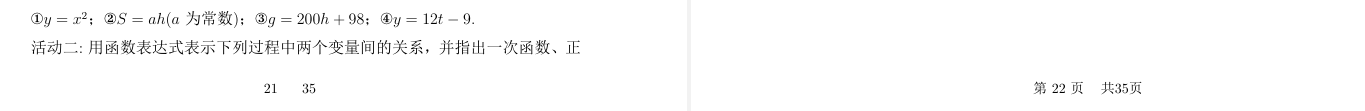
\includegraphics[width=\textwidth]{figure/chap-text/pifontconflict.png}
    \caption{页脚中文不显示}
\end{figure}

\qaq{解决方法:}参考\href{https://github.com/CTeX-org/ctex-kit/issues/688}{pifont宏包可能会触发中文不显示},把\lstinline{\makexeCJKactive}加到页眉页脚的开头。
\begin{lstlisting}
    \fancyfoot[C]{  \songti 第\thepage 页  \hspace{0.5em} 共\pageref{LastPage}页}
\end{lstlisting}

\section{脚注}\label{sec:footnote}

脚注命令:
\begin{lstlisting}
\footnote[手动指定序号,可忽略]{脚注内容}
\end{lstlisting}



\section{尾注}\label{sec:endnote}
\LaTeX{} 目前没有提供直接插入尾注的命令,但可以调用endnotes宏包实现。

不常用,暂时略过。

\section{交叉引用}\label{sec:crossref}
可以使用\lstinline|\ref|命令和\lstinline|\label|命令进行交叉引用。在正文中,使用\lstinline|\ref{label}|命令引用,在相应位置使用\lstinline|\label{label}|命令进行标记。

\section{列表}\label{sec:list}

\subsection{无序列表}\label{subsec:itemize}
无序列表环境:

\vspace{2em}
\begin{minipage}{0.45\textwidth}
    \begin{lstlisting}
        \begin{itemize}
            \item 第一项
            \item [-]第二项
            \item [*]第三项
        \end{itemize}
    \end{lstlisting}
\end{minipage}
\begin{minipage}{0.45\textwidth}
    \begin{itemize}
        \item 第一项
        \item [-]第二项
        \item [*]第三项
    \end{itemize}
\end{minipage}

条目之间间距较大,可以使用长度赋值命令将条目环境额外的垂直空白设置为0pt,达到与正文间距一致:

\begin{lstlisting}
    \itemsep=0pt
    \parskip=0pt
\end{lstlisting}


\subsection{有序列表}\label{subsec:enumerate}
有序列表环境:

\vspace{2em}
\begin{minipage}{0.45\textwidth}
    \begin{lstlisting}
        \begin{enumerate}
            \item 第一项
            \item 第二项
            \item 第三项
        \end{enumerate}
    \end{lstlisting}
\end{minipage}
\begin{minipage}{0.45\textwidth}
    \begin{enumerate}
        \item 第一项
        \item 第二项
        \item 第三项
    \end{enumerate}
\end{minipage}

有序列表可以嵌套,可对其序号、标号和前缀进行重定义,但是比较麻烦,可以使用paralist宏包。


\subsection{paralist宏包}\label{subsec:paralist}

暂未接触使用,略过。

\section{代码展示}\label{sec:codeshow}

因为\LaTeX{}排版会自动忽略空白字符等,如果需要按照原格式排版,可以使用\lstinline{verbatim}环境。


\begin{codeshow}
    不使用verbatim环境:
    int main() {
            printf("Hello, world!");
            return 0;
        }

    使用verbatim环境:
    \begin{verbatim}
        int main() {
            printf("Hello, world!");
            return 0;
        }
    \end{verbatim}
\end{codeshow}

行内可以使用\lstinline{\verb|内容|}。

也可以使用\lstinline{lstlisting}宏包。可以实现复杂的高亮效果,但需要额外的配置。
